% Chapter Template


\chapter{Results and Discussion}

\label{Chapter6:Results}

%----------------------------------------------------------------------------------------
% Transfer learning
% effect of loss function
% effect of camera intrinsic 
% effect of Hyper parameter
% Effect of recreating holes.. 
 
 
%----------------------------------------------------------------------------------------
In this chapter we have evaluated your system and presented a comparative results  based on different experimental setup discussed in section \ref{Chapter5:Methodology}. We have categorized our experiments into 3 different sections as shown in the table below \ref{table:Results_main} to investigate in three difference areas. This table lists all the experiments carried out for this study on depth estimation. In the following sections we will be describing our results mentioned in the table and will be discussing about it in its respective sections.  We have 3 accuracy values based on different threshold namely (a1, a2, and a2) and two error metrics namely root mean square error (rms) and log\_10 error as mentioned in section. Experiments \textbf{E1} and \textbf{E2} where performed to understand the importance of structural dependency of depth maps and to test our proposed model against the state of the art system. In experiments \textbf{E3} and \textbf{E4} we validate the influence of different camera intrinsic properties over data from structure sensor, by this we can also see the influence of transfer learning even when trained on different dataset with different feature properties. Experiments \textbf{E5} and \textbf{E6} was carried out to study behaviour of probabilistic distribution over the invalid pixel which we call it as holes, this leads us to answer the question of efficient way for depth estimation.

 
% Please add the following required packages to your document preamble:
% \usepackage{multirow}
\begin{table}[h]
\begin{tabular}{p{0.05\linewidth}p{0.3\linewidth}p{0.1\linewidth}p{0.1\linewidth}p{0.08\linewidth}p{0.08\linewidth}p{0.07\linewidth}}
\hline
\textbf{\#} & \textbf{Model} & \multicolumn{3}{l}{\textbf{Accuracy}} & \multicolumn{2}{l}{\textbf{Error}} \\ \cline{3-7} 
                    &                        & a1       & a2       & a3      & RMSE         & log\_10      \\ \hline
\multicolumn{7}{l}{\texttt{Influence of Structural Characteristics}}                                            \\ \hline
\textbf{E1}                  &  \textbf{A1}  & 0.22         & 0.43          &  0.61       & 0.34            &   0.001           \\ \hline
\textbf{E2}                  & \textbf{A2}  &    0.60  & 0.859 & 0.93       &   0.19          &0.11              \\ \hline
\multicolumn{7}{l}{\texttt{Influence Of Transfer Learning}}                                                                   \\ \hline
\textbf{E3}                  & \textbf{A2\_Holes}(N+S)              & 0.39   & 0.58   & 0.65  & 0.27      & 1.70       \\ \hline
\textbf{E4}                  & \textbf{A2\_Holes}(S) & 0.33   & 0.55   & 0.63  & 0.34      & 1.78       \\ \hline
\multicolumn{7}{l}{\texttt{Holes Regeneration}}                                                       \\ \hline
\textbf{E5}                  & \textbf{A2\_NoHoles}            & 0.98   & 0.98   & 0.98  & 0.10       & 0.18        \\ \hline
\textbf{E6}                  & \textbf{A2\_Holes}              & 0.39   & 0.58   & 0.65  & 0.27      & 1.70       \\ \hline
\end{tabular}

\caption{This table list all the results of experimental configuration performed. These experiments are grouped in to three categories. In E3, (N+S) denotes that model trained on NYU\_v2 and SD, where as in E4, (S) denotes model trained on SD\V2}
\label{table:Results_main}
\end{table}

\newpage

\section{Influence of Structural Characteristics}
 \begin{figure}[h]
\settoheight{\tempdima}{\includegraphics[width=.32\linewidth]{example-image-a}}%
\centering\begin{tabular}{@{}c@{ }c@{ }c@{ }c@{}}
&\textbf{RGB} & \textbf{Truth} & \textbf{Predticted} \\
\rowname{E1 (a)}&
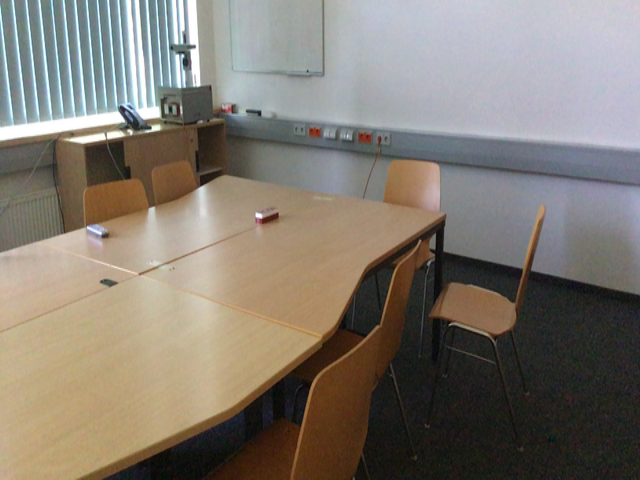
\includegraphics[width=.3\linewidth]{Figures/results/s1_a1/u0RAW_RGB.png}&
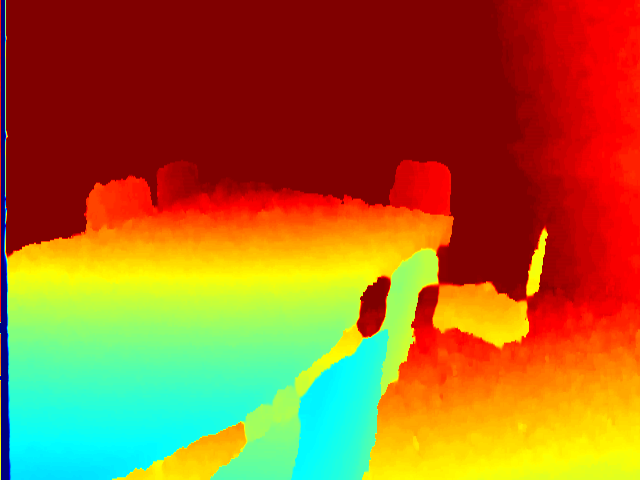
\includegraphics[width=.3\linewidth]{Figures/results/s1_a1/u0Truth.png}&
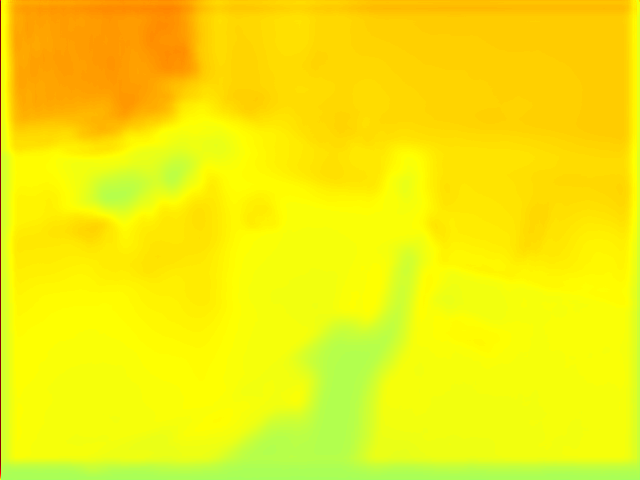
\includegraphics[width=.3\linewidth]{Figures/results/s1_a1/u0Predicted.png}\\[-1ex]
\rowname{E2 (b)}&
\includegraphics[width=.3\linewidth]{Figures/results/s1_a1/0RAW_RGB.png}&
\includegraphics[width=.3\linewidth]{Figures/results/s1_a1/0Truth.png}&
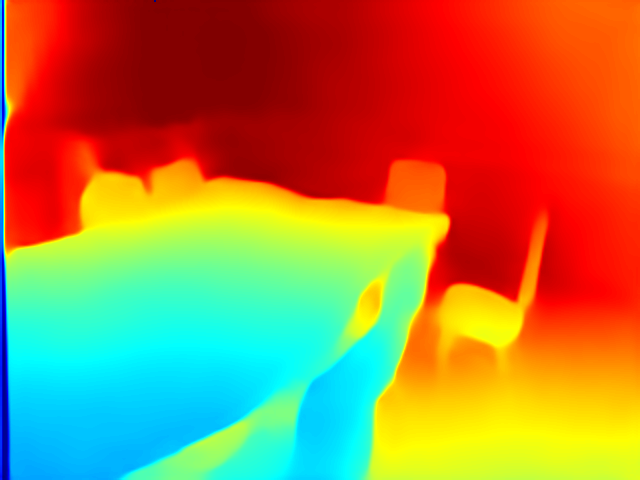
\includegraphics[width=.3\linewidth]{Figures/results/s1_a1/0Predicted.png}\\[-1ex]
\end{tabular}
\caption{\textbf{Influence of Structural Characteristics:} All the \textbf{E3} methods are in different  }%
\label{fig:results_E1_E2}
\end{figure}

\label{Chapter6:Influence_Structural_Char}
In this section we have investigated the Influence of Structural Characteristics of a pre-trained network backbone. \textbf{E1 - A1} model has no previously trained weights whereas \textbf{E2- A2} model has DenseNet backbone with pre trained weights only for the encoder part, which means, by evaluating \textbf{E1 - A1} against \textbf{E2 - A2} we can find out wheather the pre-trained backbone encoder model can have a influence over our results. One main significant different is in the decoder block, \textbf{A2} model is not trained on ImageNet as we discussed earlier in Section \ref{Chapter3:RelatedWork_NNModel} which implies the \textbf{A2} encoder has learnt Structural Characteristics feature from RBG images. Therefor we evaluate this influence of such pre-trained backbone. Therefore we train both the models with same SD\_v1 dataset with the train, validation and test set split of 80\%, 10\%  and 10\% respectively. Note that in \textbf{E2 - A2} case, we train only the decoder part. From the result in table \ref{table:Results_main} we see that the model performs gives a accuracy \textbf{a1} of only \textbf{0.22} which is 22 \% when compared with \textbf{A2} accuracy of \textbf{0.60}. Also the RMSE error is also high in \textbf{E1 - A1} compared to \textbf{E2 - A2}. Similarly the output from both the model in fig. \ref{fig:results_E3_E4} also shows  \textbf{E1 - A1} failed to perform. Important factor to notice is that, there were several layer parameters and hyper parameters where changed and tested before reaching the current \textbf{E1 - A2}. Due to the poor performance we did not document every step of model tuning of \textbf{E1 - A1} 

Observation: On a positive note for \textbf{E1 - A1} there are two things to be noted. First,  \textbf{E1 - A1} model can learn some structure characters as seen in the predicted image in fig. \ref{fig:results_E3_E4} \textbf{E1(a)} we notice that the chair could be identified to be closer than the wall behind. Second, we noticed that training and prediction is relatively  faster than \textbf{E2 - A2} model which means smaller network can give faster results. On the negative  side performance is very poor. 
Therefore, it is very clear that \textbf{E2 - A2} with DenseNet backbone outperforms \textbf{E1 - A1}. Since the accuracy of \textbf{E1 - A1} was extremely poor we believe that this is an effect of less data available for training, which gave us an motivation for SD\_v2  dataset to generate more data. Thus we believe for further experiments choosing \textbf{A2} model over \textbf{A1} would be beneficial. Which leads us to the second step of this study which is to answer, if we can train the network to reproduce the holes in the similar fashion to Structure Sensor. And we have a better working model \textbf{A2} but still not the best. Since as we see in Fig. \ref{fig:results_E1_E2} the sooth edges around the objects in the predicted frame. 
 


 

 \section{Effect of Camera Properties}
 \label{Chapter6:Transfer_Learning}
Second investigation was performed to find the influence of transfer learning. In this method we input depth image for the network was with holes, still keeping the primary objective in this second stage of experimental process of finding optimal model for the best results. In order to find the best working model, From the previous investigation we understood the impact of pre-trained backbone (encoder) in our case which is DenseNet, in this experiment we two different configuration changes only on decoder part by keeping the encoder unchanged. Initially in first experiment \textbf{E3 - A2\_Holes(N+S)}  we trained our decoder part with two datasets one from kinect sonsor (NYU\_v2) and Structure sensor (SD\_v2)and in the second experiment \textbf{E4 - A2\_Holes(S)} we only with Structure sensor (SD\_v2) dataset. By this we can study the effects and influence different camera properties in our results there by achieving optimal model for our task.

The results from the table \ref{table:Results_main} we notice that all the three accuracy of \textbf{E3 - A2\_Holes(N+S)} is higher than \textbf{E4 - A2\_Holes(S)} similarly both the error is also lower for \textbf{E3 - A2\_Holes(N+S)} which means \textbf{E3 - A2\_Holes(N+S)} perform better than  \textbf{E4 - A2\_Holes(S)}. But when we compare difference of these five metrics individually, we find that there are only small difference. For instance lets us consider RMSE, \textbf{E3 - A2\_Holes(N+S)} has error rate of \textbf{0.27} while \textbf{E4 - A2\_Holes(S)} error rate is \textbf{0.34} with difference \textbf{0.07}. In the same way for accuracy \textbf{a1}, the accuracy difference between both the configurations where only \textbf{0.06}, for \textbf{a2} is \textbf{0.03} and for \textbf{a3} is just \textbf{0.02}. 

But when we compare the resultant depth maps from these two experimental configurations, visually the difference are higher with respect to precision at the object boundaries which can be seen in the Fig.\ref{fig:results_E3_E4}  where \textbf{E3 (a) - E3(c)} represented the resultant output from \textbf{E3 - A2\_Holes(N+S)} and similarly  \textbf{E4 (a) - E4(c)} represented the output from \textbf{E4 - A2\_Holes(S)}. We notice two significant difference, first a blurred effect at object edges for the model trained only on SD\_v2 dataset, where as we get refined edges with \textbf{E4 - A2\_Holes(S)}. Secondly, we observe that our model \textbf{E3 - A2\_Holes(N+S)} has learnt the holes. What is more interesting is as we see in the Fig. \ref{fig:results_E3_E4} \textbf{E3 (b)} model can learn even the complex environment which is comprised of many pole looking structures (legs of chairs in a classroom environment).

Oservation: As we have seen that our \textbf{A2} model when trained with both dataset performs better than when trained on one dataset alone. On a positive note, we see that data from Kinect sensor has improved our results. On the other hand, when we consider the size of SD\_v2 compared with NVU\_v2, SD\_v2 is relatively small. So it is difficult to study and conclude the effect of camera properties. But what we can say is NYU\_v2 dataset has a significant impact in our result and our current model can be trained to higher precision even for regeneration of holes.



 
 \begin{figure} [h]
\settoheight{\tempdima}{\includegraphics[width=.32\linewidth]{example-image-a}}%
\centering\begin{tabular}{@{}c@{ }c@{ }c@{ }c@{}}
&\textbf{RGB} & \textbf{Truth} & \textbf{Predticted} \\
\rowname{E3 (a)}&
\includegraphics[width=.3\linewidth]{Figures/results/s2_Holes/0RAW_RGB.png}&
\includegraphics[width=.3\linewidth]{Figures/results/s2_Holes/0Truth.png}&
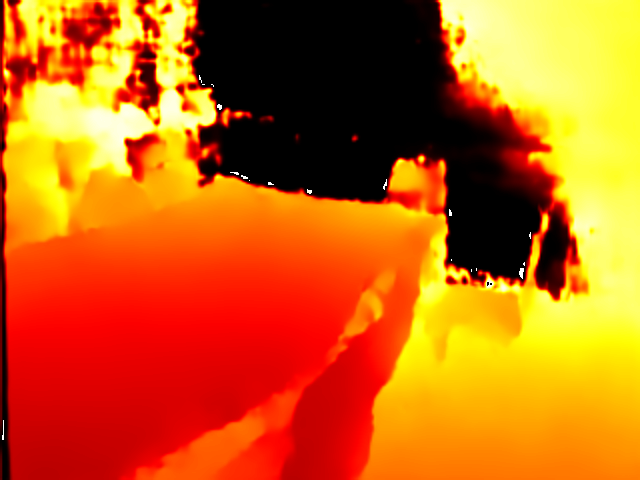
\includegraphics[width=.3\linewidth]{Figures/results/s2_Holes/0Predicted.png}\\[-1ex]
\rowname{E3 (b)}&
\includegraphics[width=.3\linewidth]{Figures/results/s2_Holes/1RAW_RGB.png}&
\includegraphics[width=.3\linewidth]{Figures/results/s2_Holes/1Truth.png}&
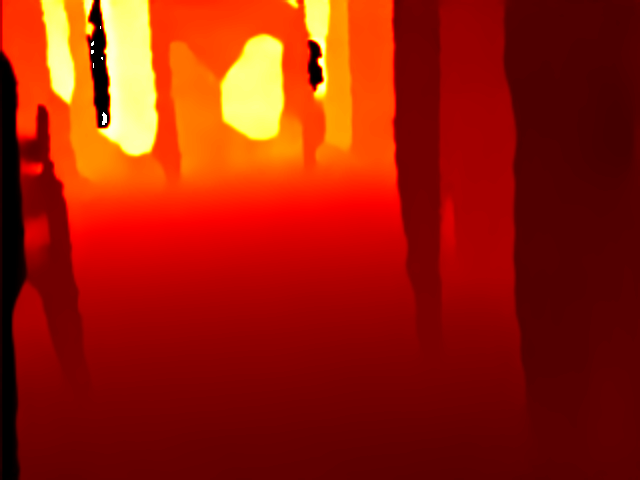
\includegraphics[width=.3\linewidth]{Figures/results/s2_Holes/1Predicted.png}\\[-1ex]
\rowname{E3 (c)}&
\includegraphics[width=.3\linewidth]{Figures/results/s2_Holes/2RAW_RGB.png}&
\includegraphics[width=.3\linewidth]{Figures/results/s2_Holes/2Truth.png}&
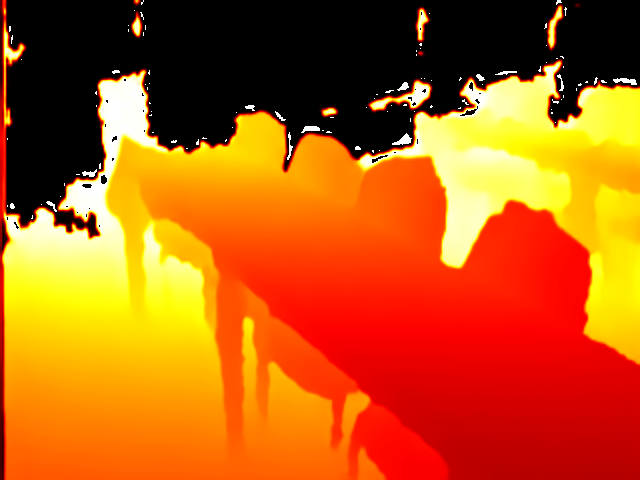
\includegraphics[width=.3\linewidth]{Figures/results/s2_Holes/2Predicted.png}\\[-1ex]
\rowname{E4 (a)}&
\includegraphics[width=.3\linewidth]{Figures/results/s3_noNyu/0RAW_RGB.png}&
\includegraphics[width=.3\linewidth]{Figures/results/s3_noNyu/0Truth.png}&
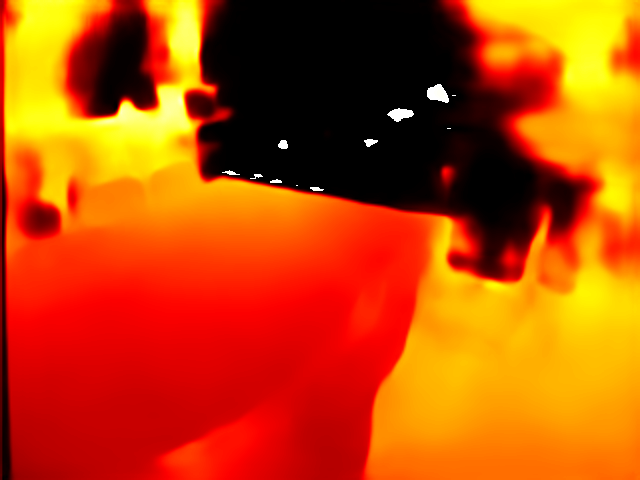
\includegraphics[width=.3\linewidth]{Figures/results/s3_noNyu/0Predicted.png}\\[-1ex]
\rowname{E4 (b)}&
\includegraphics[width=.3\linewidth]{Figures/results/s3_noNyu/1RAW_RGB.png}&
\includegraphics[width=.3\linewidth]{Figures/results/s3_noNyu/1Truth.png}&
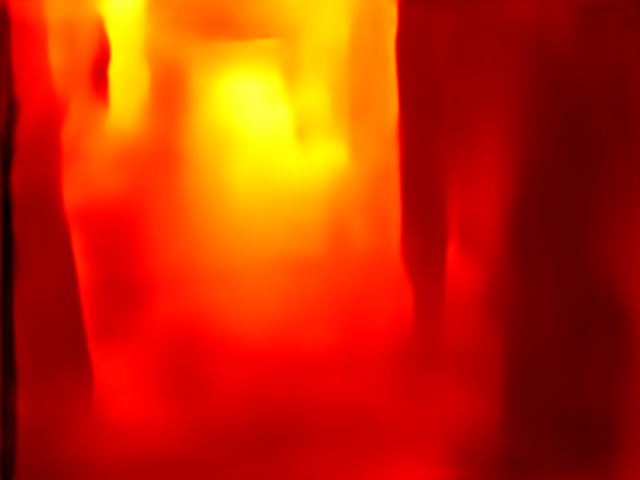
\includegraphics[width=.3\linewidth]{Figures/results/s3_noNyu/1Predicted.png}\\[-1ex]
\rowname{E4 (c)}&
\includegraphics[width=.3\linewidth]{Figures/results/s3_noNyu/2RAW_RGB.png}&
\includegraphics[width=.3\linewidth]{Figures/results/s3_noNyu/2Truth.png}&
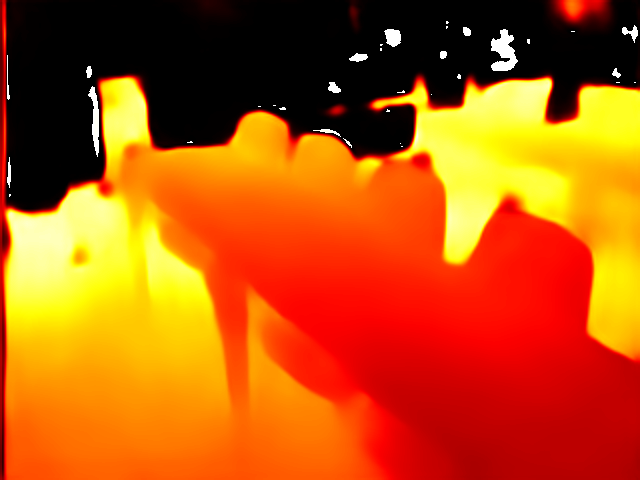
\includegraphics[width=.3\linewidth]{Figures/results/s3_noNyu/2Predicted.png}\\[-1ex]
\end{tabular}
\caption{\textbf{Investigation on hole regeneration method:} All the \textbf{E3} methods are in different  }%
\label{fig:results_E3_E4}
\end{figure}





\newpage
 \section{Hole Regeneration}
 \label{Chapter6:Hole_Regeneration}
Further more to improve the results for estimation of depth maps for 3D reconstruction, we study the importance/influence of effects of a probabilistic distribution (in other words neural network's output is a distribution of probable values ranging from 0.0 to 1.0 on a image level) over this regenerating holes. As described in section \ref{Chapter4:Dataset}, in order to have a holes recreated we mapped all the dead value or no pixel region as zero. Therefore we have two methods of pre-possessing carried out with two different input feature type, one with holes and another without holes. We tested the performance of \textbf{A2\_Holes} against the \textbf{A2\_NoHoles} models. In Fig. \ref{fig:results_S2} (a) - (c) we see that there a good reconstruction of the depth map were all the holes were interpolated to its neighboring pixel.  Fig. \ref{fig:results_S2} (d) - (f)  corresponds to the model with the holes as a input to the network. As we see in Fig \ref{fig:results_S2}, we compare \textbf{E5} and \textbf{E6}. We have used two different color maps for \textbf{E5} and \textbf{E6}. This is because in \textbf{E4} we wanted to highlight the difference between holes which were mapped to zero and the closest region in an image. 

From the table \ref{table:Results_main} we notice that the on an average the model \textbf{E3 (A2\_NoHoles)} performs better. When RMSE is taken into consideration we can clearly see that \textbf{E3 (A2\_NoHoles)} performs better with the RMSE of \textbf{0.10} which is \textbf{0.17} lower than the \textbf{E4 (A2\_Holes)} with RMSE of \textbf{0.27}. And when we notice our accuracy a1, a2 and a3 we see the similar results when compared. But when notice in the Fig. \ref{fig:results_S2} (d) - (f) we have visually good prediction. when investigated further why such hugh difference in the accuracy and error we found out the error lies in the object boundaries. As we see in the fig () there is a interpolation intermediate pixel from the zero value (holes which are mapped as zeros) till the actual depth. This effect is cause because of the probabilistic distribution method of neural network characteristic. We strongly this is one of there main factors contributing to the difference in the error and accuracy between \textbf{E5} and \textbf{E6}. Now that we understand why such effects can be seen for the generation of holes, it is very important us to answer if such approach is beneficial or not. Given such a problem of linear \notice{interpolating prediction} one possible solotion can be given by some post-filtering or post processing methods but the idea for the case of this study is to provide end to end approch as much as possible thereby exploiting the potential of the neural network. 

Therefore we see that given an input with holes the model can learn the holes from the given monocular input. But it results into \notice{interpolating prediction} which we believe makes the 3D reconstruction of a scene more difficult and demands further post processing techniques. This leads us to an conclusion that interpolating of pixel is a better approach than making the network learn to predict holes. In addition to this, one of the other motivation to try this approach was to eliminate the wall effect of depth maps  for the pixel farther than the distance limit, one approach for this solution could be taking a threshold just before the highest pixels. This solves the problem of having wall in out 3D reconstruction scene.

In summary, we believe that the comparing the two different input representation, \textbf{A2\_NoHoles} approach where the holes are interpolated with its neighboring pixels is beneficial.





\begin{figure} 
\settoheight{\tempdima}{\includegraphics[width=.32\linewidth]{example-image-a}}%
\centering\begin{tabular}{@{}c@{ }c@{ }c@{ }c@{}}
&\textbf{RGB} & \textbf{Truth} & \textbf{Predticted} \\
\rowname{E3 (a)}&
\includegraphics[width=.3\linewidth]{Figures/results/s2_NoHoles/0RAW_RGB.png}&
\includegraphics[width=.3\linewidth]{Figures/results/s2_NoHoles/0Truth.png}&
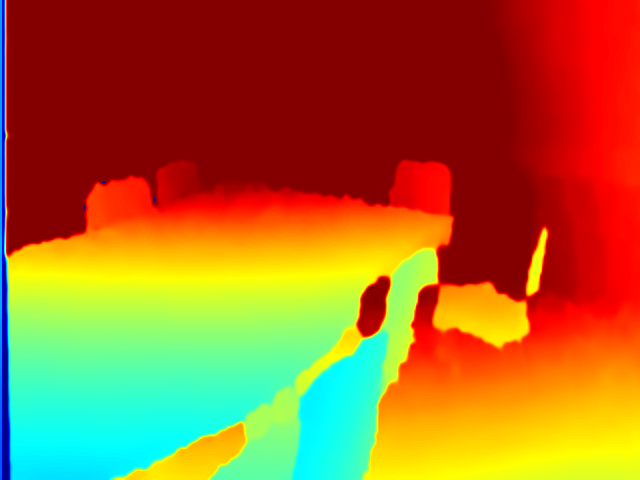
\includegraphics[width=.3\linewidth]{Figures/results/s2_NoHoles/0Predicted.png}\\[-1ex]
\rowname{E3 (b)}&
\includegraphics[width=.3\linewidth]{Figures/results/s2_NoHoles/1RAW_RGB.png}&
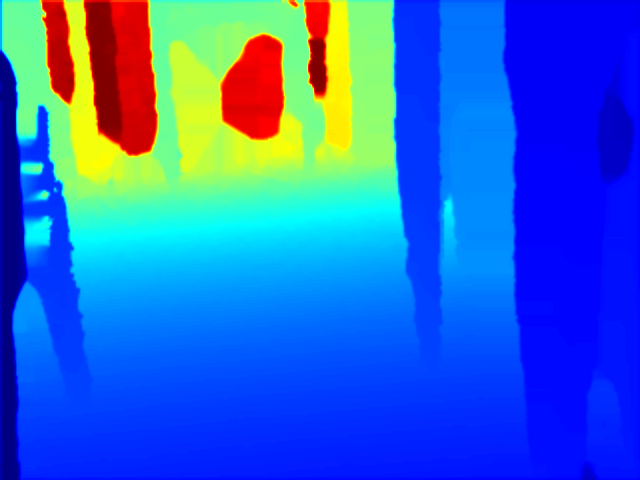
\includegraphics[width=.3\linewidth]{Figures/results/s2_NoHoles/1Truth.png}&
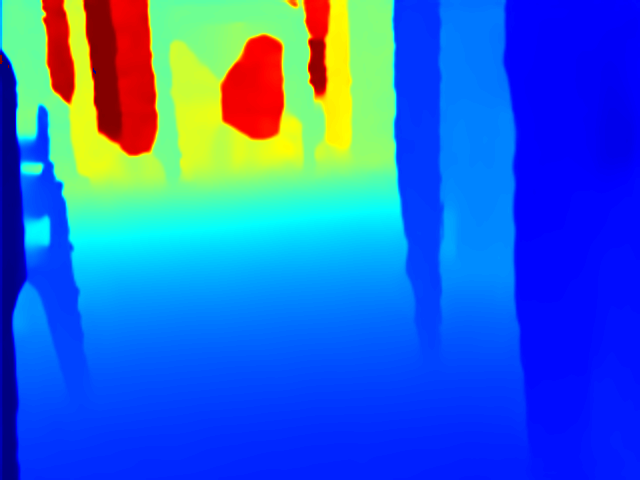
\includegraphics[width=.3\linewidth]{Figures/results/s2_NoHoles/1Predicted.png}\\[-1ex]
\rowname{E3 (c)}&
\includegraphics[width=.3\linewidth]{Figures/results/s2_NoHoles/2RAW_RGB.png}&
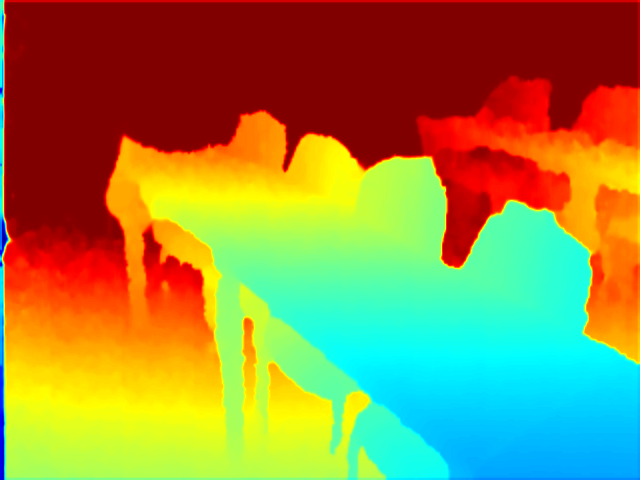
\includegraphics[width=.3\linewidth]{Figures/results/s2_NoHoles/2Truth.png}&
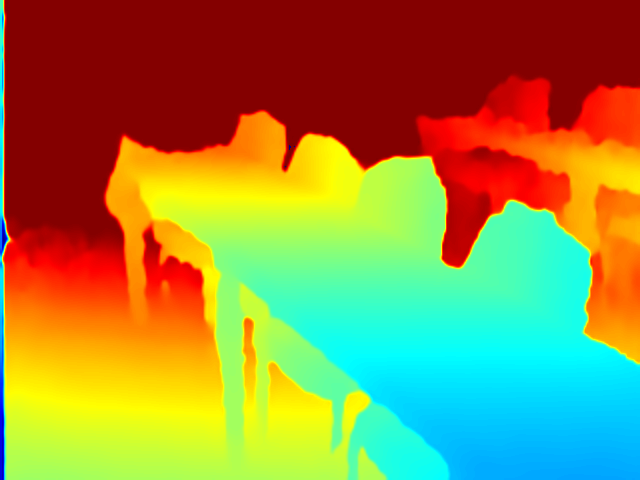
\includegraphics[width=.3\linewidth]{Figures/results/s2_NoHoles/2Predicted.png}\\[-1ex]
\rowname{E4 (d)}&
\includegraphics[width=.3\linewidth]{Figures/results/s2_Holes/0RAW_RGB.png}&
\includegraphics[width=.3\linewidth]{Figures/results/s2_Holes/0Truth.png}&
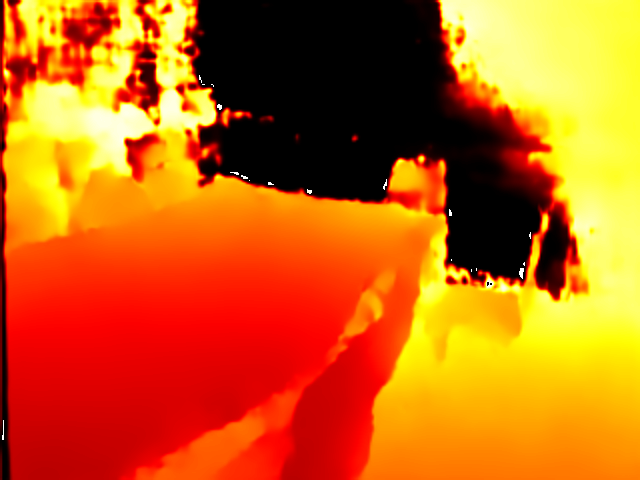
\includegraphics[width=.3\linewidth]{Figures/results/s2_Holes/0Predicted.png}\\[-1ex]
\rowname{E4 (e)}&
\includegraphics[width=.3\linewidth]{Figures/results/s2_Holes/1RAW_RGB.png}&
\includegraphics[width=.3\linewidth]{Figures/results/s2_Holes/1Truth.png}&
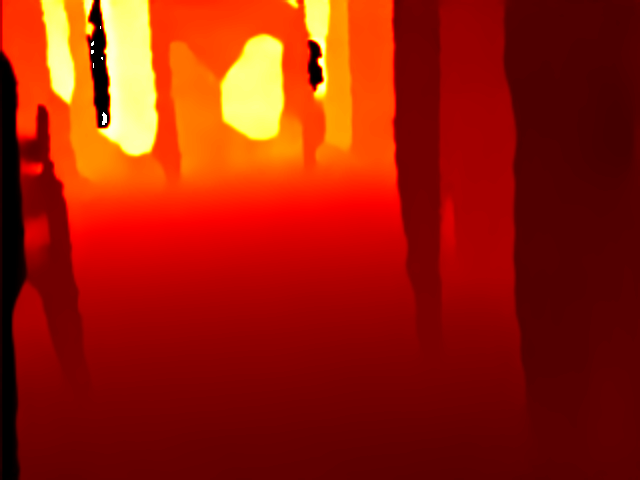
\includegraphics[width=.3\linewidth]{Figures/results/s2_Holes/1Predicted.png}\\[-1ex]
\rowname{E4 (f)}&
\includegraphics[width=.3\linewidth]{Figures/results/s2_Holes/2RAW_RGB.png}&
\includegraphics[width=.3\linewidth]{Figures/results/s2_Holes/2Truth.png}&
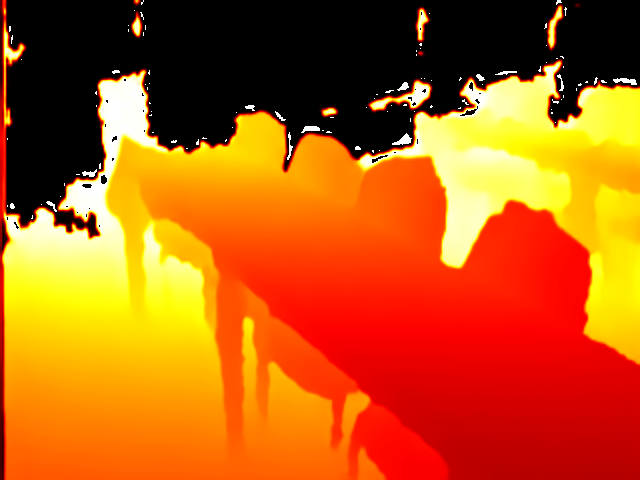
\includegraphics[width=.3\linewidth]{Figures/results/s2_Holes/2Predicted.png}\\[-1ex]
\end{tabular}
\caption{\textbf{Investigation on hole regeneration method:} All the \textbf{E3} methods are in different  }%
\label{fig:results_S2}
\end{figure}





%\section{Qualitative evaluation}

%Here we have evaluted our result with the state of the art in the table below